\documentclass[../main.tex]{subfiles}
\begin{document}

\setcounter{footnote}{0} 


\chapter{Introduction}

Advances in the chemical sciences are essential if the world is to meet the United Nations Sustainable Development Goals by 2030\cite{UN-SDGs} and prevent potentially catastrophic and irreversible climate change.\cite{IPCCwarming} With most chemicals encountering a catalyst en-route to their final form,\cite{Roduner2014} enhancing catalytic activity and selectivity lowers the energy demand and associated waste products. Furthermore, `circular'  synthesis -- reusing final chemical compounds by catalytic decomposition -- will be required to reduce the ever-depleting fossil fuel feedstock.\cite{GarciaMartinez2021, Miandad2019} Optimising existing catalysts and developing new ones for as-yet inconceivable transformations is therefore of paramount importance.

\begin{figure}[h!]
	\centering
	\vspace{0.4cm}
	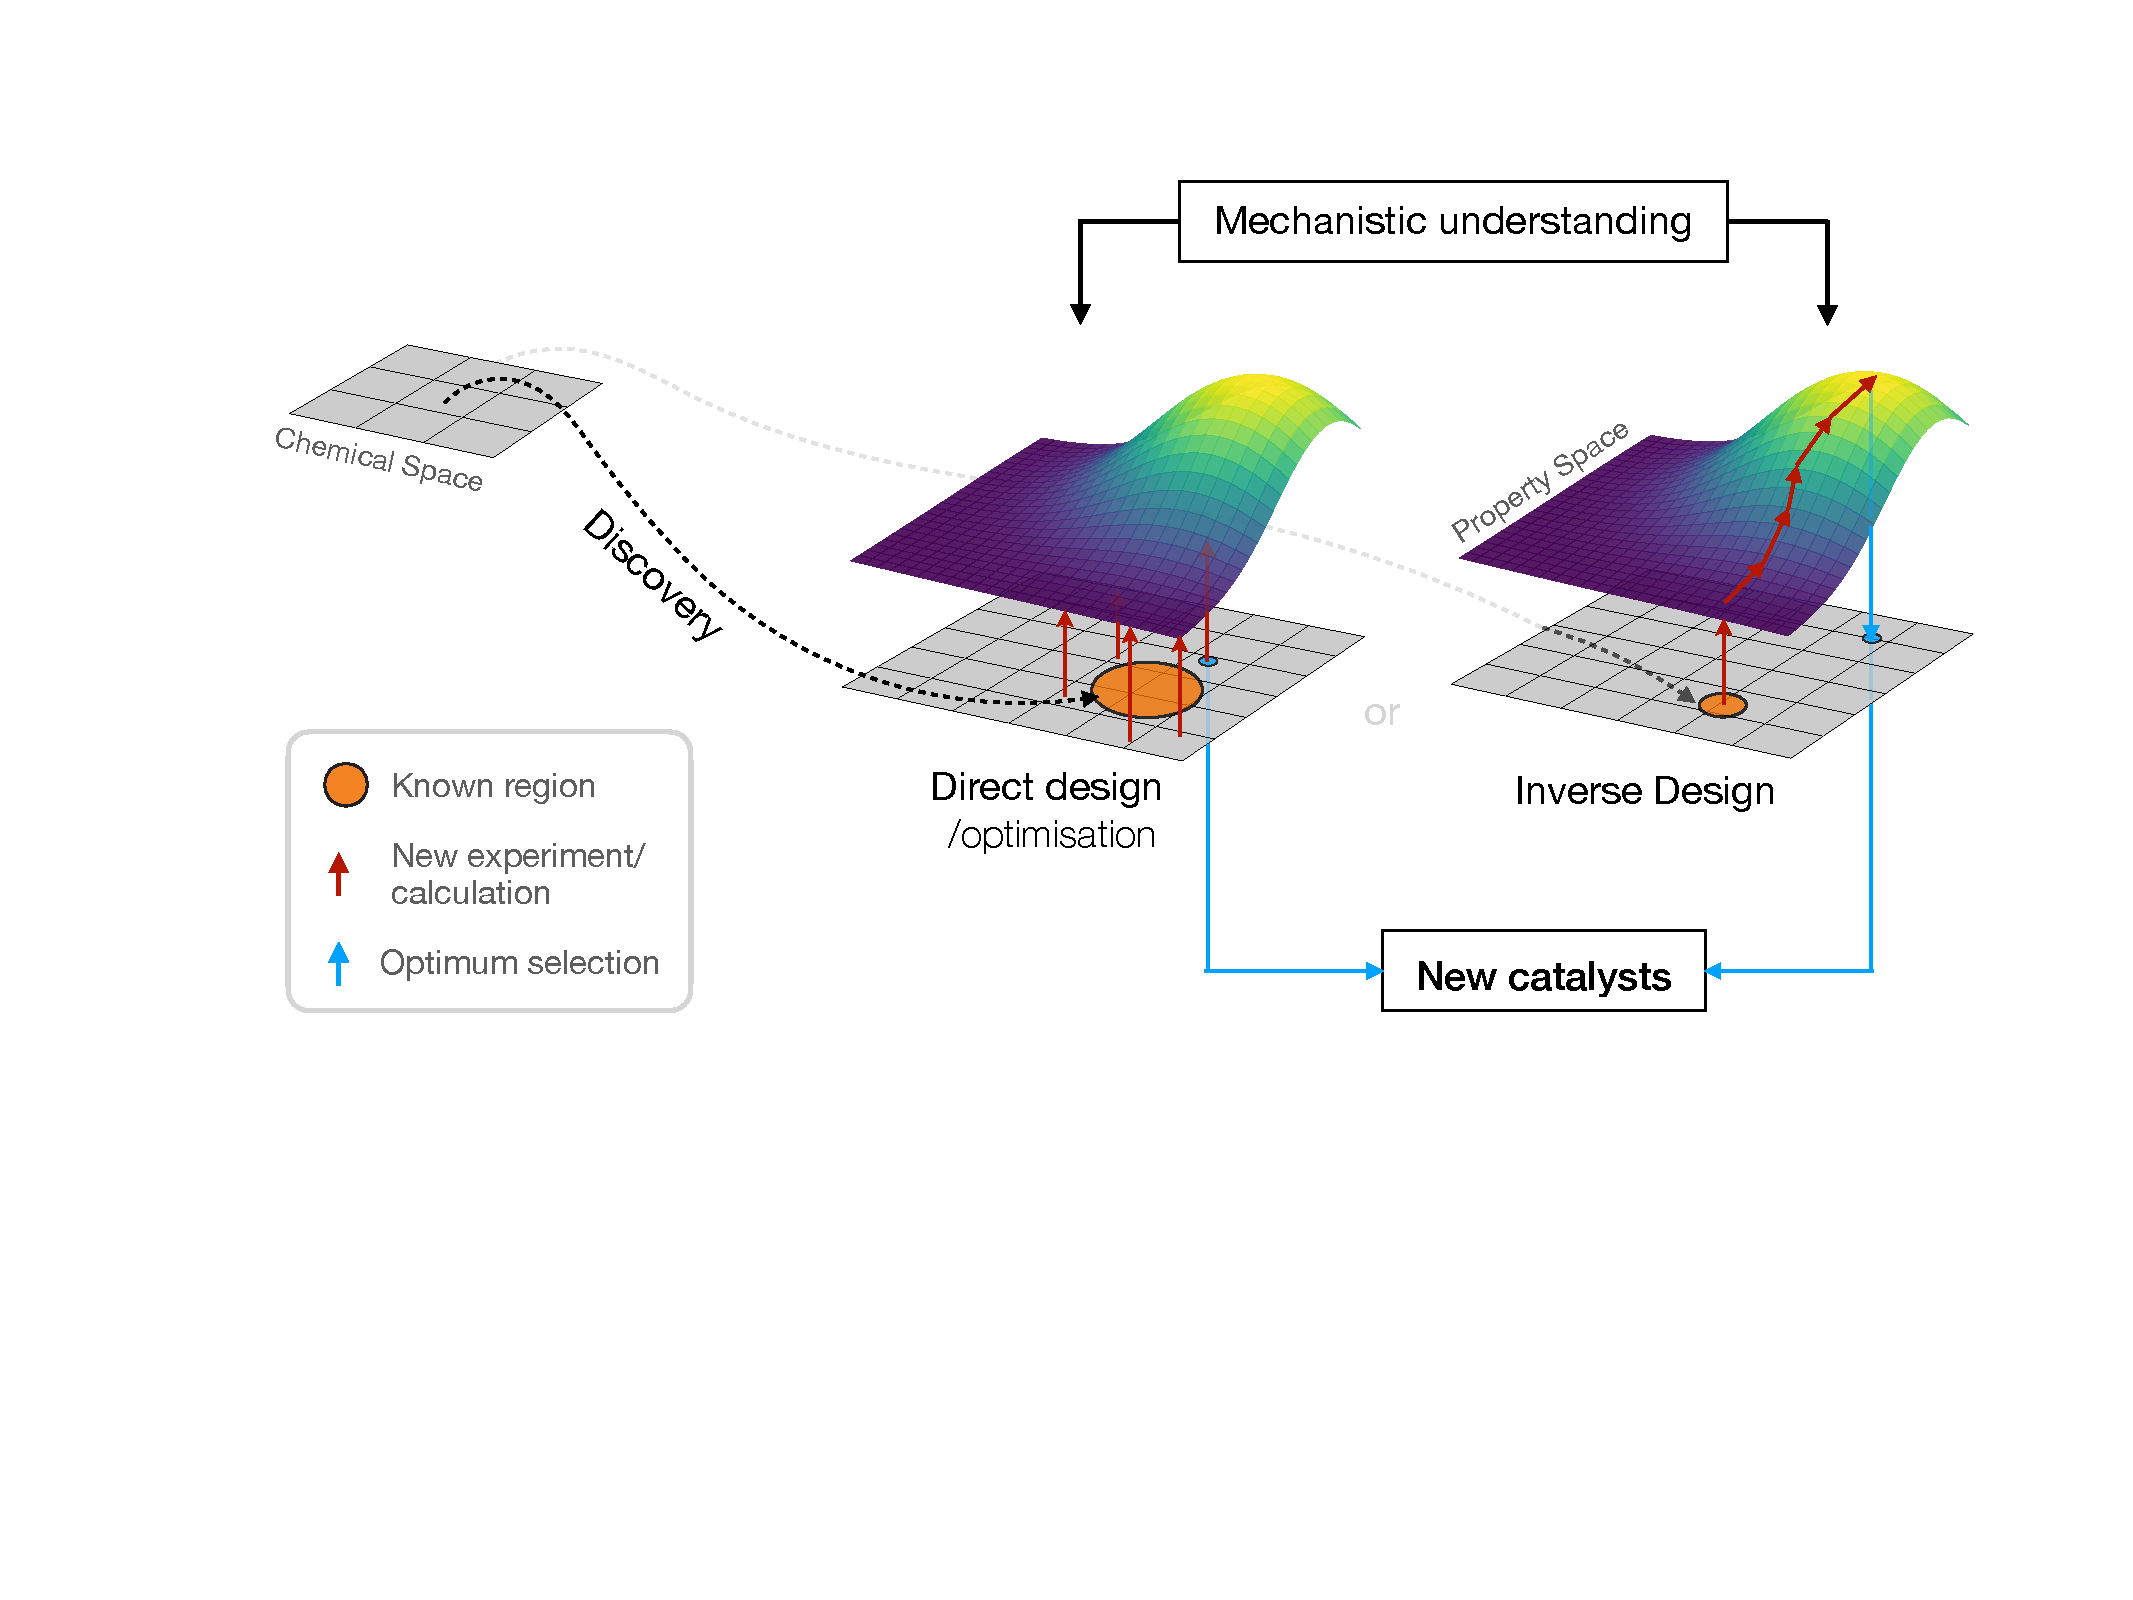
\includegraphics[width=14cm]{1/figs/fig1/intro_cat_design.pdf}
	\vspace{0.2cm}
	\hrule
	\caption{Schematic representation of the approaches to developing new catalysts.}
	\label{fig::intro_1}
\end{figure}

Discovering and optimising catalysts \emph{in-silico} is seen as somewhat of a \emph{holy-grail} in computational chemistry.\cite{Poree2017} This is because computation avoids costly experimental synthesis and testing. Strategies towards this goal will be the subject of this thesis following an overview of approaches often employed, while highlighting current limitations. \figurename{ \ref{fig::intro_1}} outlines different approaches to catalyst design, where discovery of a hit leads from an unexplored chemical space to a known region. From there, either a direct or inverse approach is generally required to optimise the hit compound to an optimal point in property space, which is then selected as a potential new catalyst. The dimensionality and complexity of the property space means a targeted approach is required, which may be aided by mechanistic understanding. These stages are expanded upon in the following sections.


\section{Discovery}

Serendipity often plays a role in discovering catalysts and their pre-requisite reactions in the experimental laboratory.\cite{Nicolaou2014, McNally2011} While high-throughput approaches are starting to be used,\cite{McNally2011, Troshin2017, Ahneman2018} a more targeted and less wasteful approach is highly desirable.

Computational methods that discover reactions and catalysts can be broadly divided into two categories: graph-based and simulation-based.\cite{Meisner2019, Dewyer2017} In the former, a graph representation is defined using atoms as  nodes and `bonds' as edges, new structures can be found from a reactant state by applying edge edits and searching for stable products (\figurename{ \ref{fig::intro_X3}}).\cite{Habershon2016, Ismail2019, Robertson2019, Kim2018, Lee2020pccp, McDermott2021} Despite being an efficient way to explore new chemical space, they are limited to discovering reactions rather than catalysts due to an exponential scaling with system size.

Simulation-based approaches employ enhanced\footnote{Standard equilibrium dynamics only sample close to the minima in currently accessible timescales (pico- to microseconds) and not over significant energy barriers ie. the rare event problem.\cite{Gerardo2009}} reactive dynamics and are also currently limited to reaction rather than catalyst discovery. Once such method is meta-dynamics developed by Parrinello in the early 2000s,\cite{Laio2002} non-equilibrium molecular dynamics\cite{Yang2019} can traverse reaction barriers on the picosecond timescale (\figurename{ \ref{fig::intro_X3}}b). These include the global reaction route mapping method,\cite{Maeda2013} which has been used to discover reaction intermediates\cite{Uematsu2015, Yoshimura2017} reactions by biasing the total energy with harmonic-like terms to find new minima. Imposed activation and conformer searching has also been used to discover reactions.\cite{Lavigne2020} These approaches apply some bias in the sampling to target `active' atoms within bonds that break or form, thus narrowing the search space. 

Methods that don not require defining `active' atoms include the ``\emph{ab initio} nanoreactor"\cite{Wang2014}, which uses high temperature dynamics under an oscillating biasing potential to favour bond formation. Adding a biasing potential to already visited regions in the configuration space has also been used to discover plausible transformations.\cite{Grimme2019} 


\begin{figure}[t!]
	\centering
	\vspace{0.4cm}
	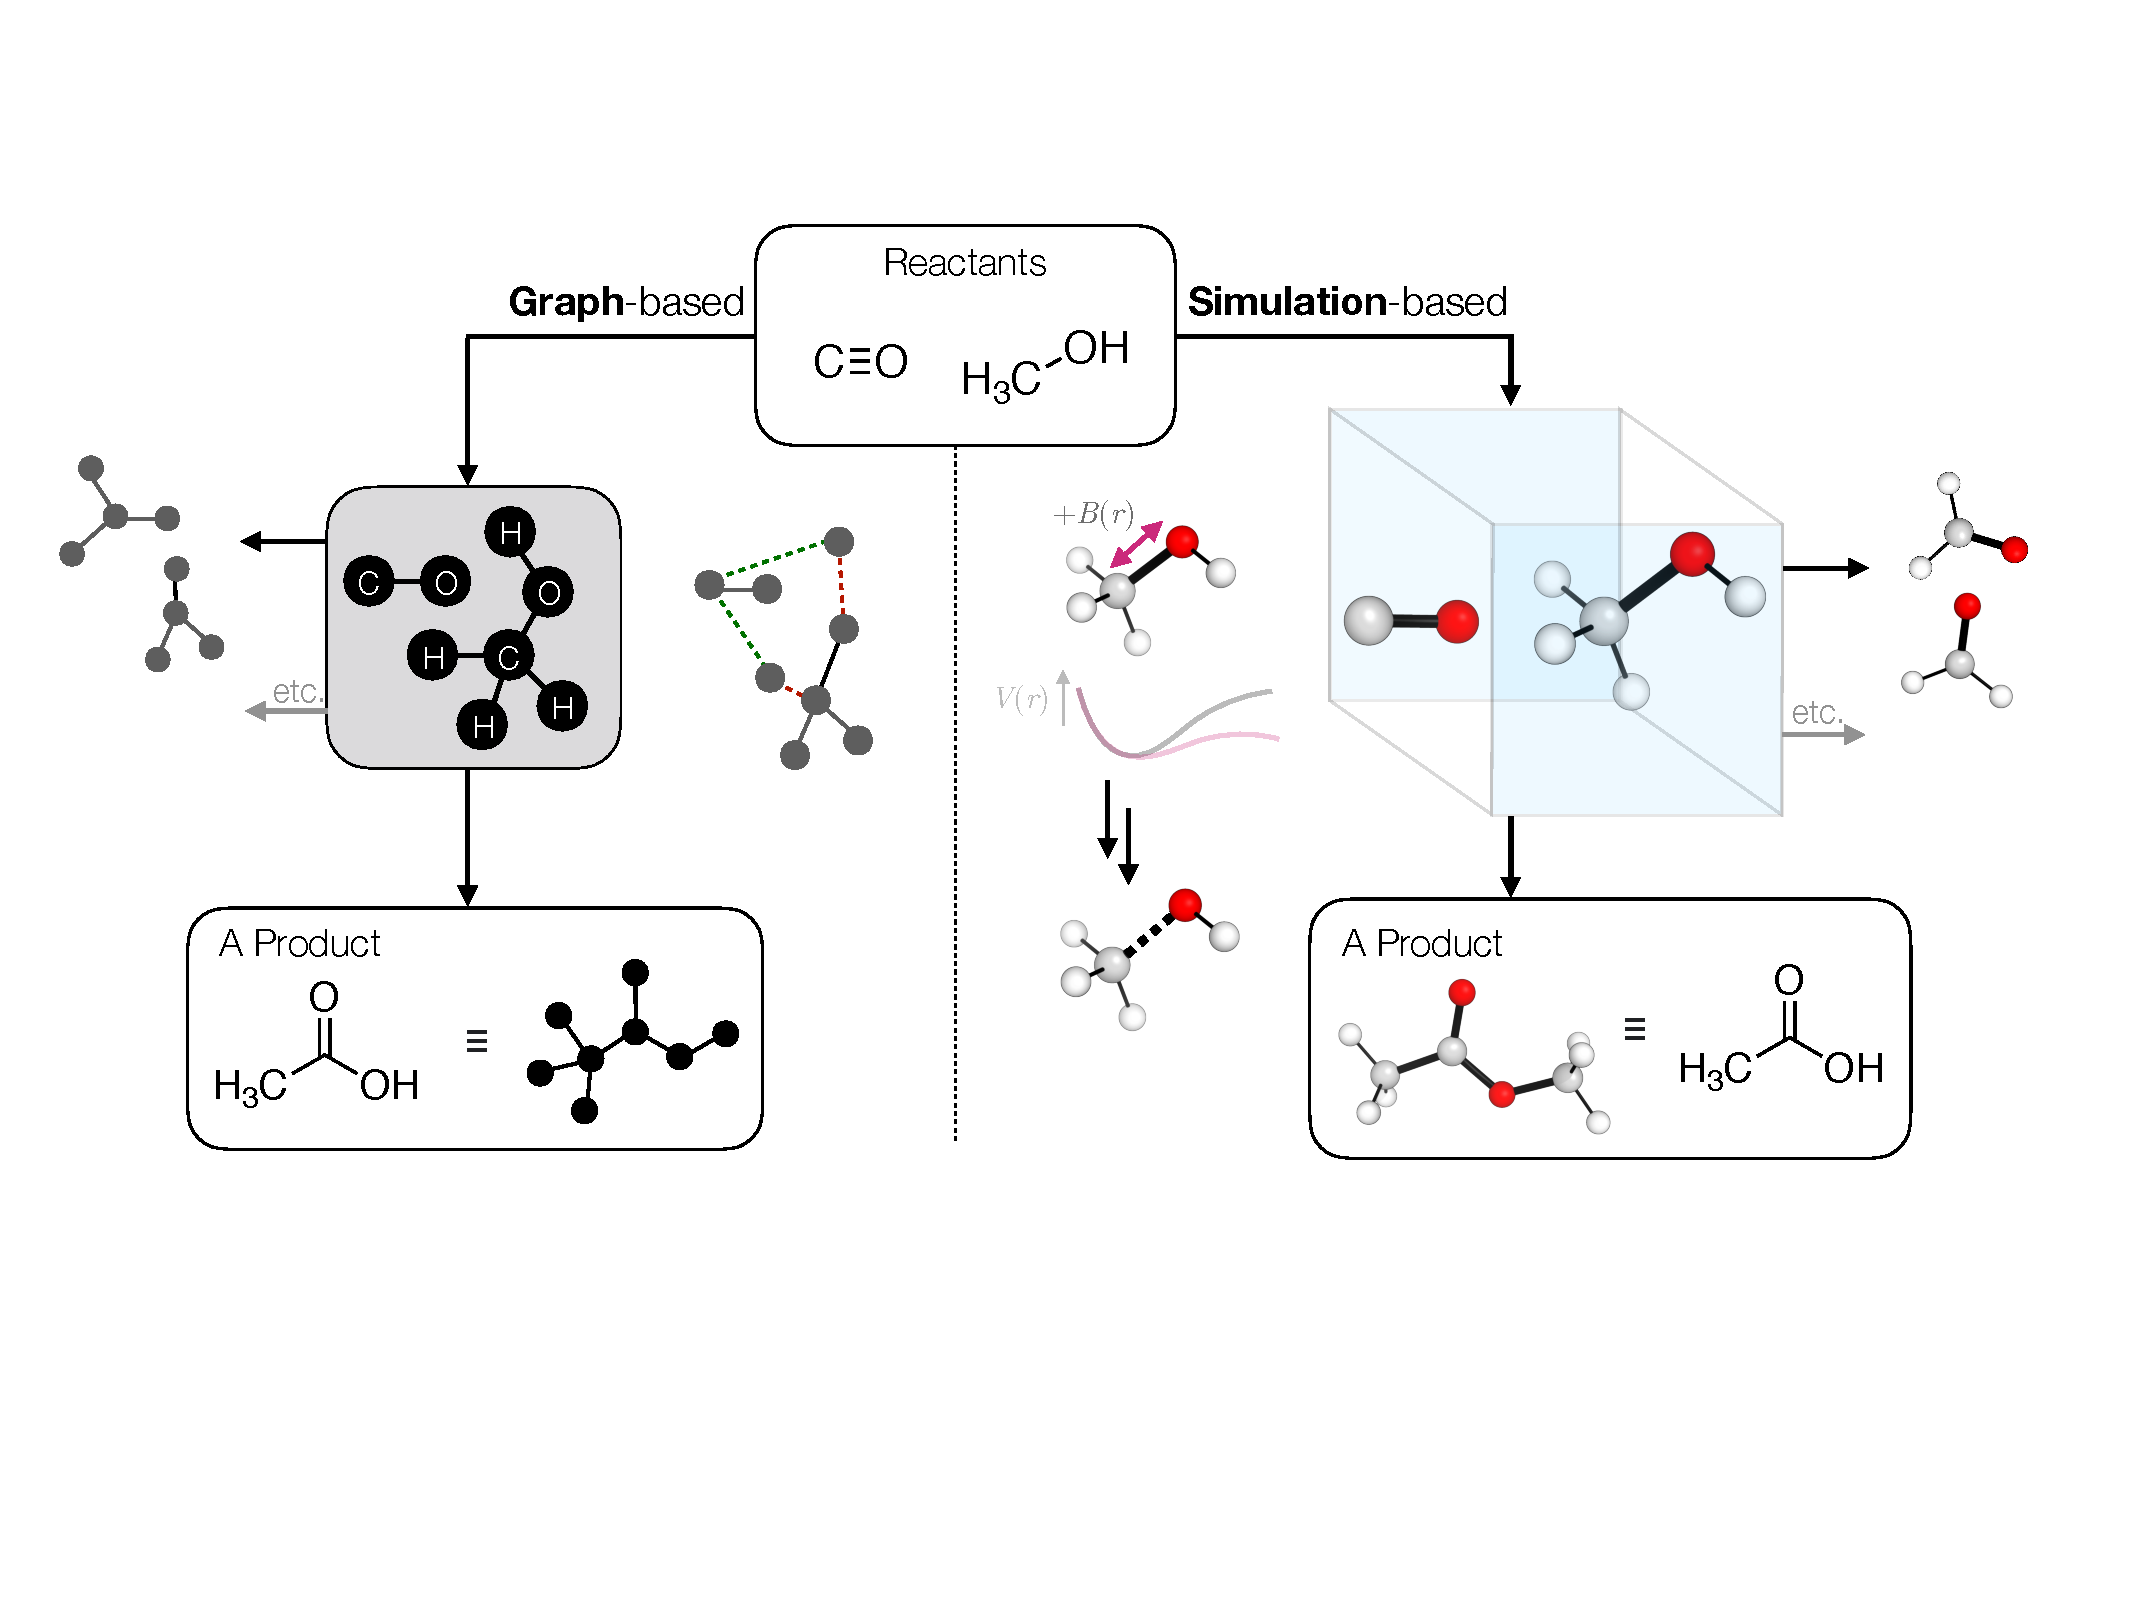
\includegraphics[width=14cm]{1/figs/fig2/fig2.pdf}
	\vspace{0.4cm}
	\hrule
	\caption{Representation of graph- and simulation-based approaches to discover new reactions between carbon monoxide and methanol. $B(r)$ is a biasing potential.}
	\label{fig::intro_X3}
\end{figure}

A comparison of these approaches is illustrated in \figurename{ \ref{fig::intro_X3}}; from a carbon monoxide and methanol mixture both methods can generate an acetic acid product but neither can suggest a catalyst. Including, for example, a transition metal and a section of ligands with a view to discovering a catalyst, leads to an intractably complex problem. 

Indeed, despite the efficiency of current computational approaches, to the best of my knowledge, a catalyst has yet to be discovered computationally without prior knowledge. Enhancing the speed and accuracy of computational methods will prove an important step towards tackle catalyst discovery, which will be the focus of this thesis.

\section{Direct-design and Optimisation}

Once a catalyst has been discovered, modification to enhance selectivity/activity is generally driven by experimental observation. Optimisation involves the reaction conditions (temperature/solvent etc.) and the catalyst identity, and while linked, the two are often considered separately. Selection of reaction conditions beyond the standard trial-and-error approach using previous experimental data is a promising approach,\cite{hase2021gryffin, Shields2021} but is still limited by experimental throughput to at most hundreds of reactions.\cite{Koinuma2004, Mennen2019} \emph{In silico} optimisation of reaction conditions without prior knowledge is an extremely challenging problem, whereas catalyst optimisation by substructure modification is currently achievable. Methods towards this are outlined in the following sections.

\subsection{Ab initio Methods}

Perhaps the simplest approach to catalyst optimisation is to modify a canonical catalyst and enumerate all possibilities within a library, calculating a relevant observable or proxy, and selecting the optimum. Although more common in drug discovery,\cite{Kitchen2004} endeavours along the same lines are being developed. For example, the \emph{AARON} (An Automated Reaction Optimizer for New Catalysts) tool has been used to exhaustively sample modified catalyst structures in organometallic complexes.\cite{Guan2018} In a similar vein, the \emph{CatVS} tool has been developed to predict enantioselectivities using enumeration over a library of ligands and ligand conformers.\cite{Rosales2018} While direct enumeration through a library is guaranteed to find the global minimum, exponential scaling of the library prevents a high diversity. However, with mechanistic understanding of the catalytic cycle targeted enumeration is a viable option. Towards using this approach in the context of supramolecular catalysis, a method for automated \emph{in silico} construction of metallocages and their host-guest complexes is introduced in Chapter 3. 

\subsection{Data-driven Methods}

Complementary to direct calculation \emph{ab initio} are data-driven approaches, which  incorporate experimental data to build regression models. These quantitative structure activity relationships (QSAR)\cite{Muratov2020} and machine learning\cite{Toyao2019, Kitchin2018, Friederich2020} approaches have been employed widely to both understand and in some cases suggest catalyst modifications using generative models.\cite{GmezBombarelli2018} These complement classic genetic algorithms for exploring or traversing\cite{Nigam2021} a local space.\cite{goldberg1989genetic} Along with suggesting perturbations to a catalyst, machine learning (ML) models also provide an avenue to select which experiments, thus observations to collect.\cite{Henle2020, Zahrt2021} 

\section{Inverse Design}

Suggesting an optimal catalyst for a given transformation i.e. `inverse design' is perhaps the ultimate goal of computational catalyst design. In contrast to optimisation, the end-to-end prediction is unobtainable using enumeration in a chemical space of $>10^{60}$ small organic molecules.\cite{Kirkpatrick2004} Indeed, inverse optimisation has only been used in small property spaces.\cite{Freeze2019, Foscato2020} Generally, this proceeds via optimisation in a continuous representation and conversion into a suggested structure. Notable examples include: plausible nitrogen-fixating catalysts by optimising a `jacket potential' of point charges surrounding a core,\cite{Weymuth2014} and a linear combination of atomic potential approach, for optimising CO$\rightarrow$CO$_2$ catalysts.\cite{Chang2018} In the latter case a calculated activation barrier was used as the objective function and the site occupancies for different groups on a chemical core the variable parameters. 
% \cite{Dittner2018} - does not propose a new strucutre, only a new environment

The lack of examples using inverse design illustrates the difficulty of the problem; it thus remains as an ultimate goal with methods being developed towards its achievement.


\section{Understanding}

One of the most prevalent uses of computation in organo(metallic) chemistry is to understand a particular (catalytic) mechanism, with the hope that such knowledge can then be used to optimise and design new catalysts rationally.\cite{Norskov2011, Tantillo2016} Given a set of experimental observations, a catalytic cycle may be calculated and an effective energy barrier quoted along with, perhaps, a rate limiting step.\cite{Kozuch2011} From this knowledge, a human-guided approach to catalyst design can be employed using classical physical organic methods, e.g. considering inductive/resonance/steric/solvation effects to modulate kinetics, which in turn modify selectivity/activity/stability.\cite{Anslyn2006} 

A notable example of how understanding can lead to better catalysts is from the groups of Houk and List, who experimental identified a highly selective catalyst for an asymmetric Mannich reaction,\cite{Mitsumori2006} based on computational modelling (see ref. \cite{Houk2008} for  further examples).\cite{Cheong2006} Understanding reaction mechanisms via computation is also crucial in organic chemistry, which was pioneered by Houk in the 1980s\cite{Houk1986}, and more recently applied in organometallic\cite{Ardkhean2020} and biocatalytic\cite{PlanasIglesias2021} settings. 

In this context, a number of collaborative projects with experimental groups were undertaken, which sought to understand reactivity and catalysis. Broadly these projects are not included in this thesis (Manuscripts \RN{5}--\RN{10}) but have provided the motivation for methods developed here.

In particular, Manuscript \RN{1}, which forms part of  Chapter 3, centres on understanding the mechanism of (in)action of two supramolecular cage catalysts. This work attempts to address the lack of enzyme-mimicking (biomimetic) supramolecular catalysts, which is an emerging field following the early experimental work of Breslow,\cite{Breslow1998}   Sanders\cite{Sanders1998} and Rebek\cite{Santamaria1999} among others. Only a few years ago computational work lead by Harvey\cite{Daver2017, Daver2018}, Himo\cite{Brea2019} and Head-Gordon\cite{Welborn2020} has started to tackle supramolecular catalysts.

Gaining mechanistic understanding through computation is, however, often a slow process. A balance is required between speed/simplicity and accuracy, which is a focus of Manuscript \RN{1} and \RN{2} (Chapter 3). Methods to improve the accuracy of mechanistic predictions is presented in Chapter 4, wherein a novel method for calculating the entropic contribution to free energies is proposed. Automation also can lead to significant speed-ups, which is the subject of Manuscript \RN{3} and is presented as Chapter 5. For modestly sized molecular systems of 50 atoms or fewer the whole process of finding minima and transition states from a 2D chemical representation accurately is automated. Finally, to efficiently modelling dynamics and reactivity, Manuscript \RN{4} is presented as Chapter 6 and outlines a method to generate machine learned potentials efficiently for a variety of systems. These dynamical effects can be important in reactions not well described by transition state theory e.g. bifurcations.\cite{Feng2021} 


\section{Summary and Outlook}

Computational approaches have been, and continue to be, important tools in discovering, understanding and optimising catalysts. Their predictive ability is, however, far from optimal. Specifically, (1) commonly employed manual computation limits throughput; (2) observable properties are challenging to calculate, particularly solution-phase equilibria and rate constants, which rely on accurate solvent and thermal contributions to the energy; (3) gas-phase energetics have a speed accuracy trade-off that often preclude high-throughput enumeration.

\begin{figure}[h!]
	\centering
	\vspace{0.1cm}
	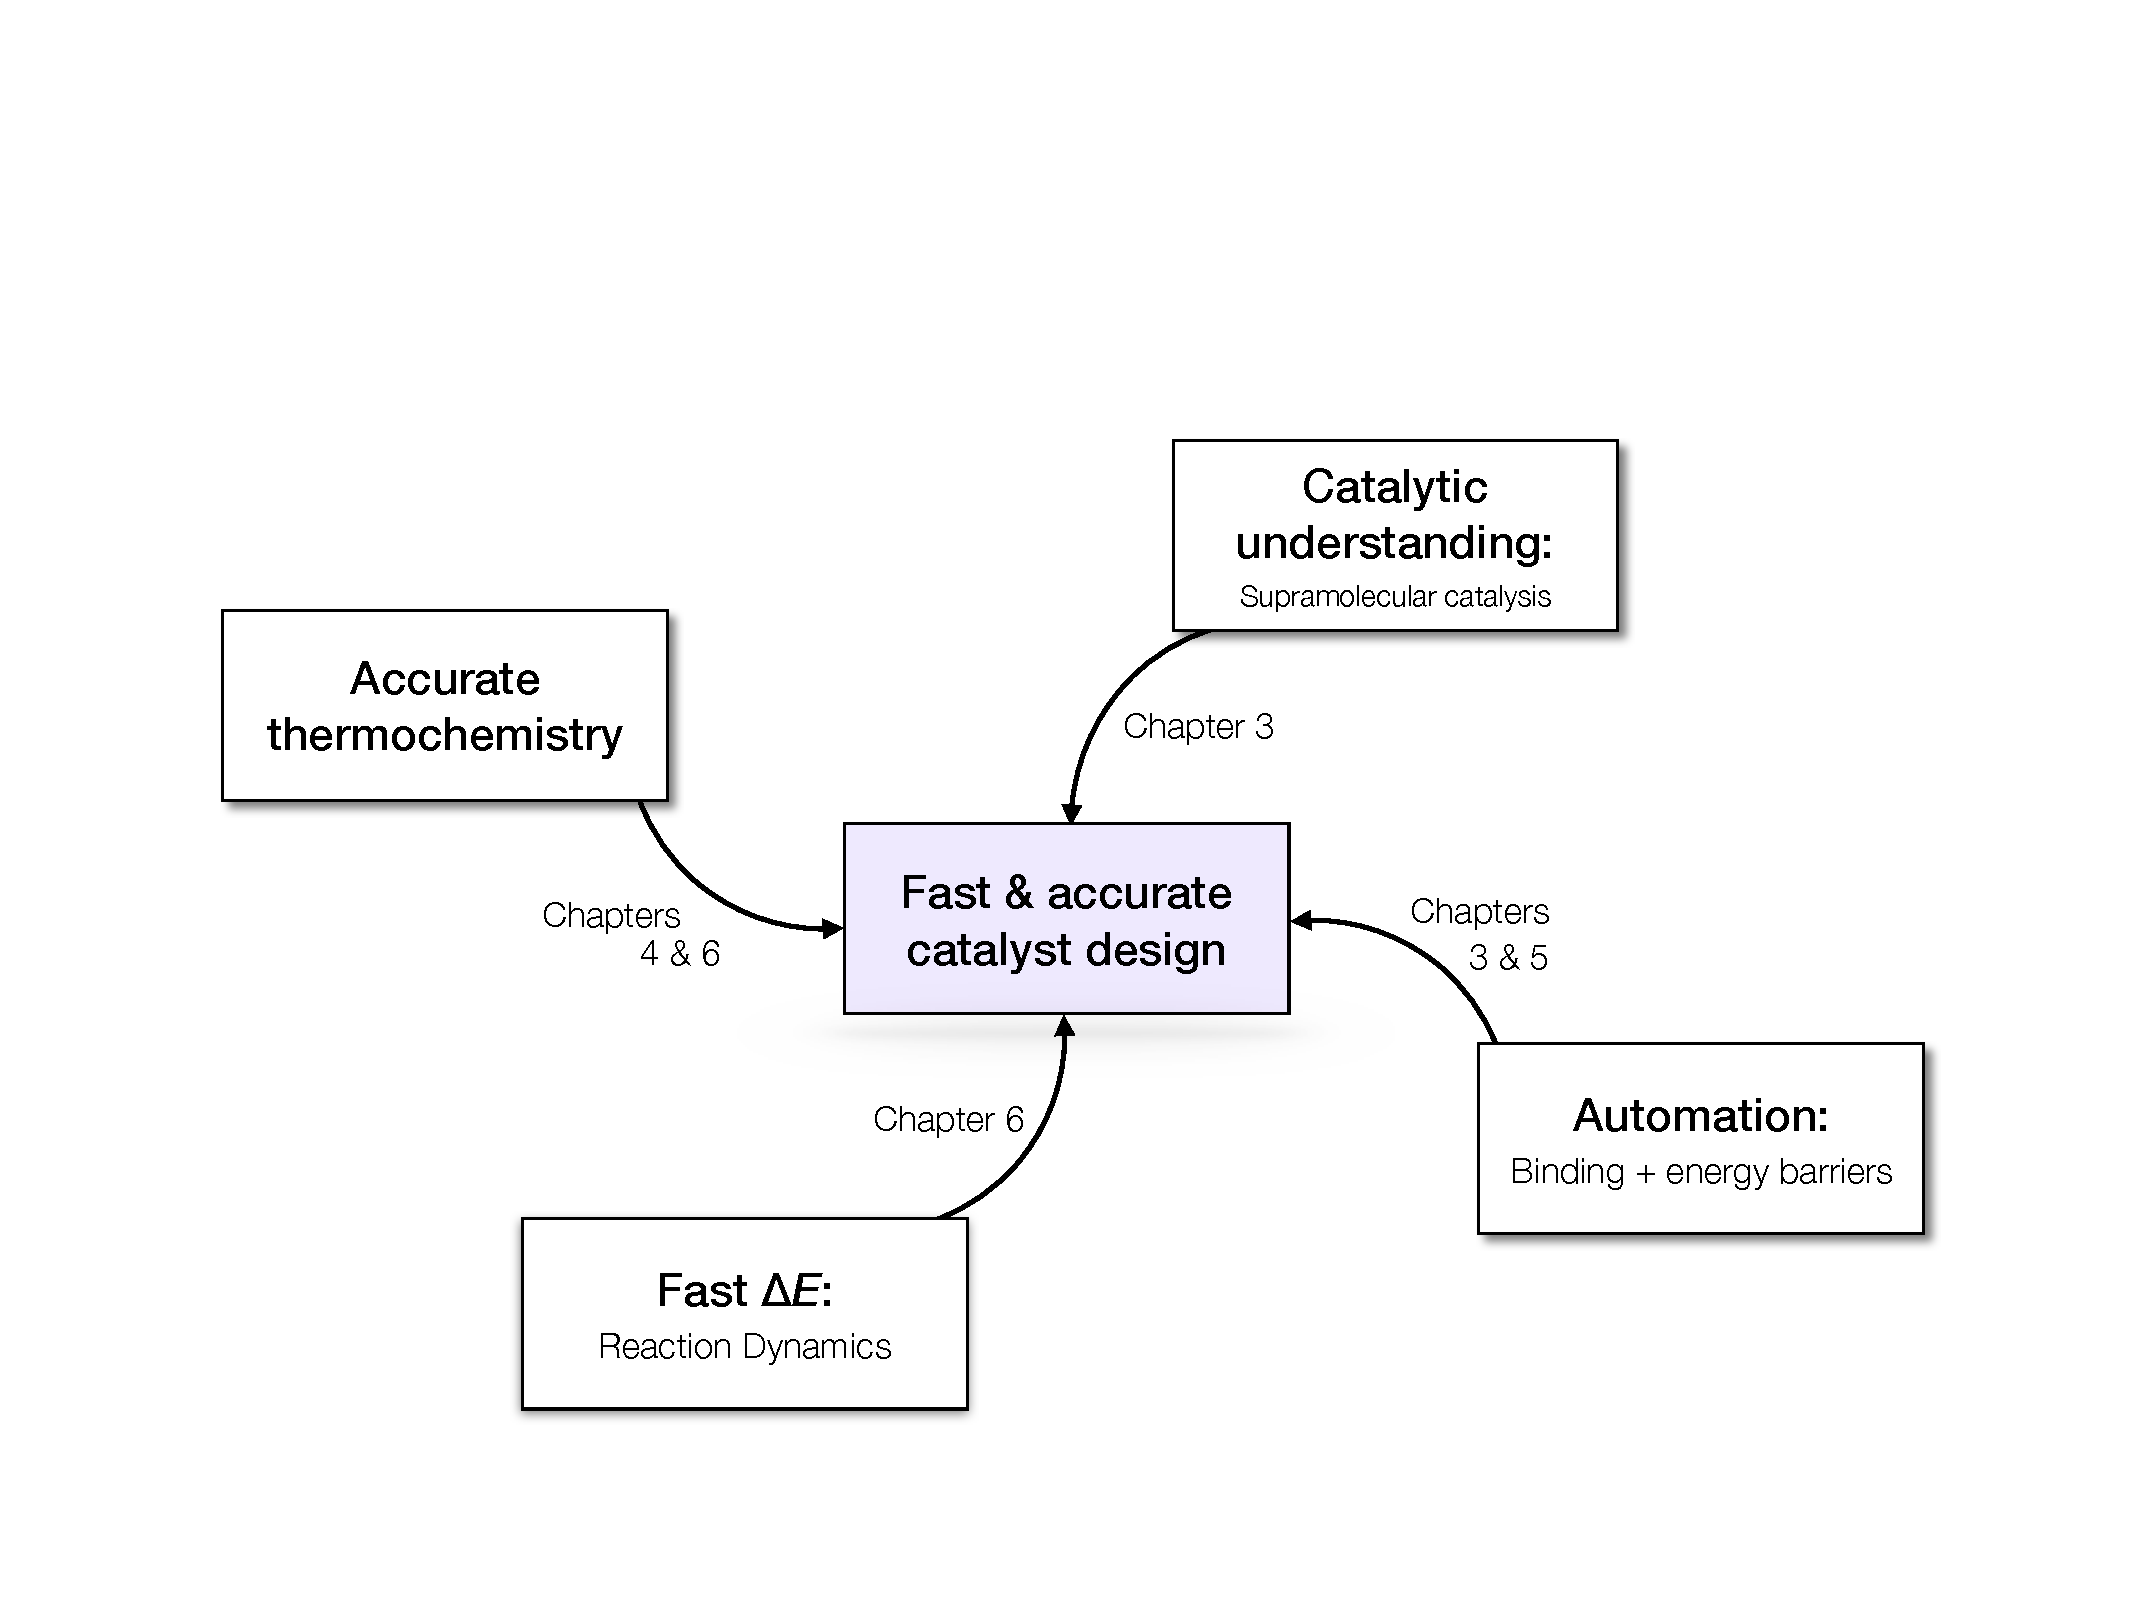
\includegraphics[width=12.5cm]{1/figs/fig3/outline.pdf}
	\vspace{0.2cm}
	\hrule
	\caption{Schematic outline of this thesis.}
	\label{fig::intro_2}
\end{figure}

Avenues in biomimetic catalysis, automation and obtaining more accurate energies from computation are the subject of this thesis and are discussed in the following chapters (Figure \ref{fig::intro_2}). From a brief theoretical background of the methods used in this thesis (Chapter 2) the first result chapter focuses on understanding a catalytic system and developing a method to enumeratively optimise it. The subsequent chapters are motivated by this work and focus largely use reactions as prerequisites to their catalytic counterparts for simplicity and speed. These methods are, however, applicable to simple catalytic processes and provide a route to developing complex catalysts computationally.





% MOre histroy




\clearpage
\end{document}